\documentclass[10pt,a4paper]{article}
\renewcommand{\baselinestretch}{1.5}
\usepackage[margin=2cm]{geometry}
\usepackage{float}
\usepackage{enumerate}
\usepackage[numbers]{natbib}
\usepackage{graphicx}
\usepackage{dcolumn}
\usepackage{bm}
\usepackage{amssymb} 
\usepackage{amsbsy}
\usepackage{amsmath}
\usepackage{color}
\usepackage{titling}
\usepackage{physics}
\usepackage{siunitx}
\usepackage{booktabs}
\usepackage{url}
\usepackage[font=small, labelfont=bf]{caption}
\usepackage{subcaption}
\usepackage{mhchem}
\usepackage[bottom]{footmisc}
\urlstyle{same}



\setlength{\droptitle}{-4cm}
\setlength{\parindent}{0pt}
\newcommand*\chem[1]{\ensuremath{\mathrm{#1}}}
\def\rf{{\ensuremath{r_{\mathrm{F}}}}}
\def\rref{{\ensuremath{r_{\mathrm{ref}}}}}
\def\rdiff{{\ensuremath{r_{\mathrm{diff}}}}}
\def\tdiff{{\ensuremath{\theta_{\mathrm{diff}}}}}
\def\tscatt{{\ensuremath{\theta_{\mathrm{scatt}}}}}

\begin{document}
	\begin{titlepage}
		\begin{center}
			\vspace*{\fill}
			{\Huge\textbf{Modelling Variability Using Hydrogen Alpha Distributions in the Galaxy}} \\
			\bigskip\bigskip {\LARGE Elliott G Charlton} \\
			\bigskip {\LARGE 18213621}\\
			\vspace{3cm}\begin{figure}[H]
				\centering
				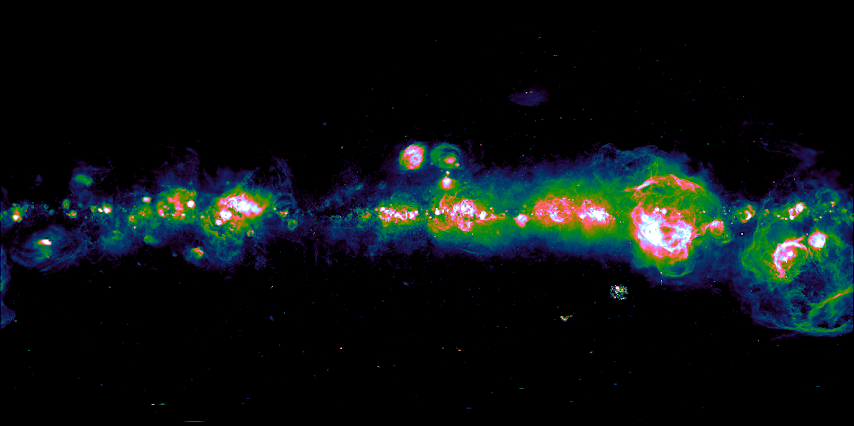
\includegraphics[width=\textwidth]{Ha1_crop}
			\end{figure}
			\vspace{3cm} {\large Honours Dissertation} \\
			\bigskip {\large Curtin University} \\
			\bigskip {\large 2018} \\
			\bigskip {\large Supervisor: Dr Paul Hancock} \\
			
			\vspace*{\fill}
		\end{center}
		\bigskip\bigskip\bigskip\vspace{\fill}
		
	\end{titlepage}
	%\maketitle
	\tableofcontents{}
	
	\newpage
	
	
\section{Literature Review}
\subsection{Abstract}
Variability is an important measure in astronomy as it can give us information about the source (intrinsic variability) or about the medium between the source and the observer (extrinsic variability). In radio astronomy the main sources that we will be observing in our images are active galaxies, and active galaxies essentially only vary extrinsically on timescales that we are observing them. We can use intensity map of H$\ce{\alpha}$ combined with a model of the structure of the galaxy and the interstellar medium to predict the amount of variability that we should observe. We want to build a model around this idea and create a program that can predict the variability of a group of sources accurately.
\subsection{The Radio Regime} \label{radio}
Since the detection of the first radio signal from Earth in the early 1930s by Karl Jansky (Jansky 1932), radio astronomy has played a key role in the advancement of our knowledge of the Universe. Before the invention of satellites, optical and radio astronomy were the prevalent branches of astronomy as these wavelengths were the only wavelengths that were not significantly blocked by the Earth's atmosphere, so that they could be observed from ground based telescopes (See Figure \ref{abs}).

\begin{figure}[H]
\begin{center}
	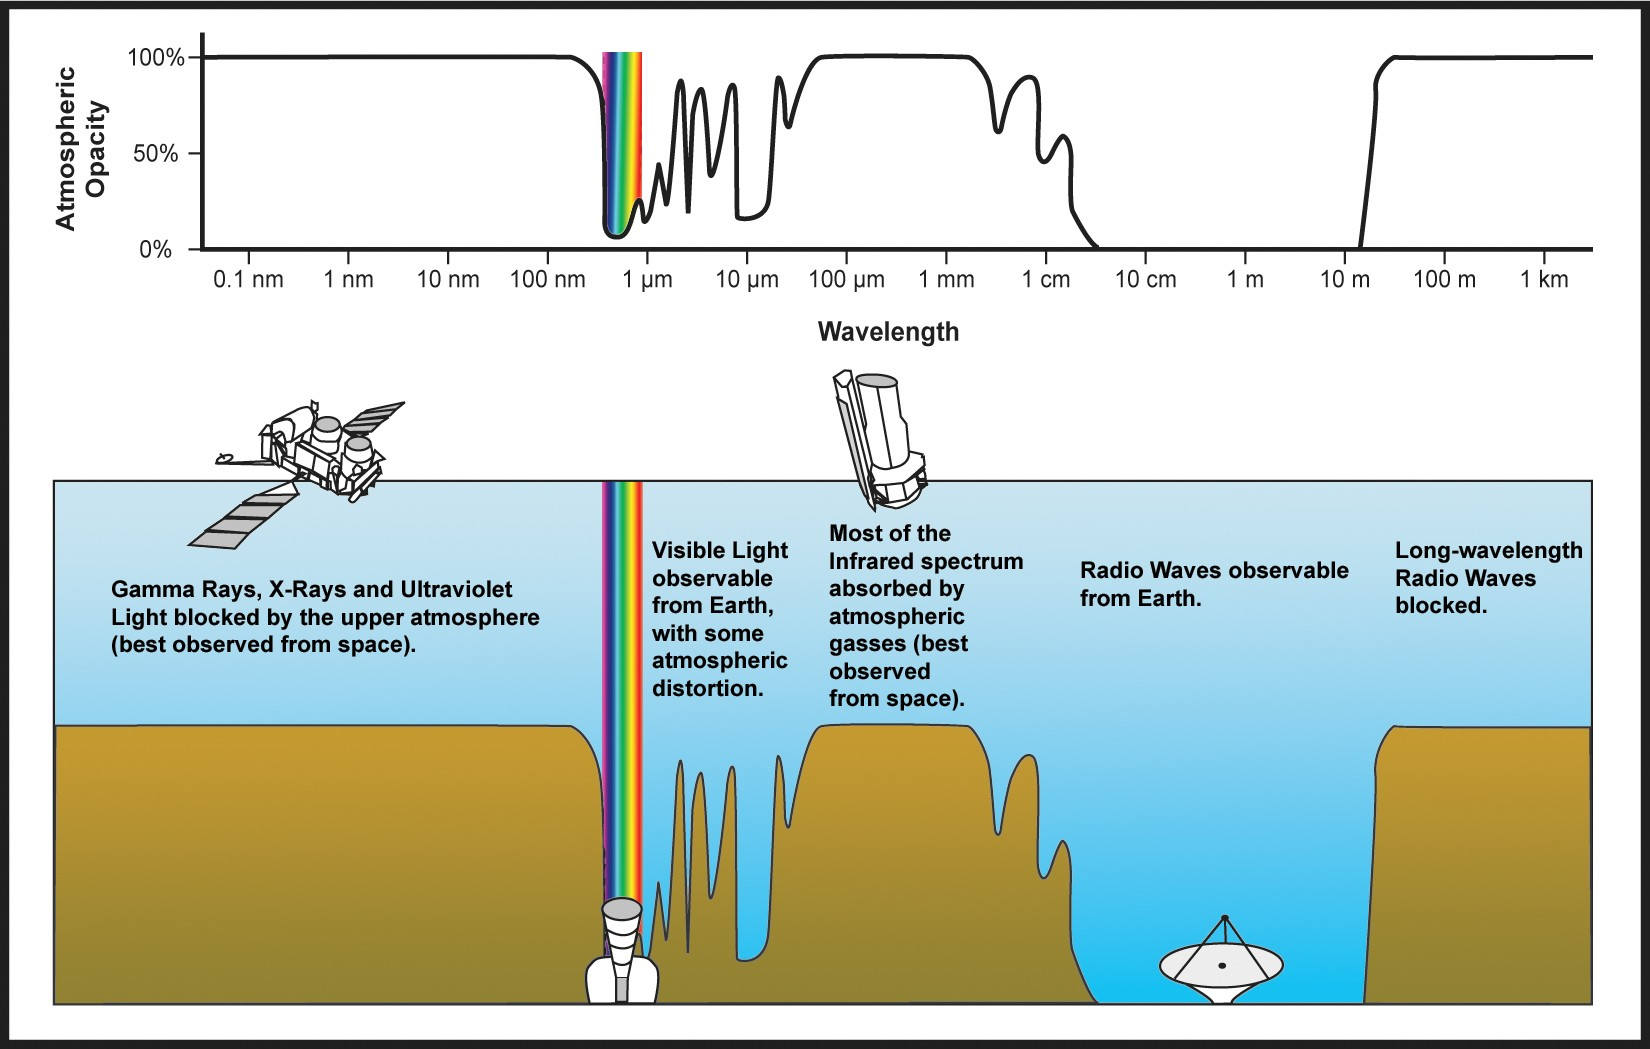
\includegraphics[width=0.75\textwidth]{atmo-abs}
	\caption{Diagram showing the blocking of different wavelengths. Most radio wavelengths can be observed from Earth\footnotemark}
	\label{abs}
\end{center}
\end{figure}
\footnotetext{\url{www.gsp.humboldt.edu/olm_2015/Courses/GSP_216_Online/lesson2-1/atmosphere.html}}
Radio wavelengths range from approximately one millimeter to ten meters ($\sim$ 30MHz - 300GHz) with the longer wavelengths being blocked by the Earths atmosphere. Typically the radio regime is observed through radio telescopes (classic parabolic dishes), and radio interferometers which are a group of telescopes that are linked together and can be used to produce higher resolution imagery. The radio emission detected by these telescopes can be grouped into two categories: line emission and continuum emission.
\subsubsection*{Line Emission}
Line emission in astronomy refers the a spectral emission line from a particular element. These lines occur due to electrons transitioning from a energy level to a lower energy level. From quantum mechanics we know that when the electron transitions between energy level it will emit a photon with energy that is equal to the energy difference between levels. From this it follows that because each element has set energy levels they will also have defined spectral lines that are unique to that elements. These lines can then be observed, an example of hydrogens electron transitions can be seen in Figure \ref{Hline}.
\begin{figure}[H]
\begin{center}
	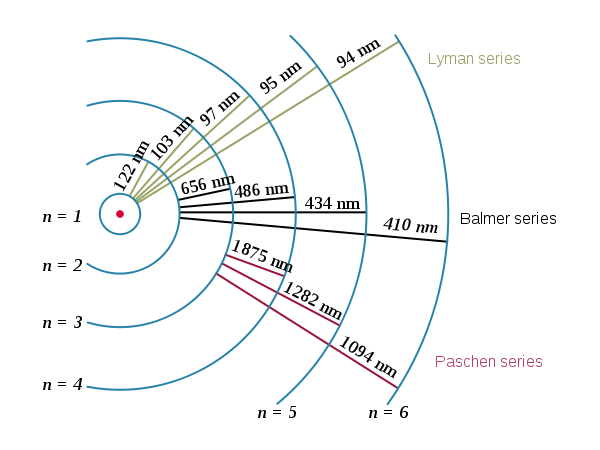
\includegraphics[width=0.8\textwidth]{Hline}
	\caption{The different electron transitions of the hydrogen element, shows up to the Paschen series\footnotemark.}
	\label{Hline}
\end{center}
\end{figure}
\footnotetext{\url{www.commons.wikimedia.org/wiki/File:Hydrogen_transitions.svg}}
From Figure \ref{Hline} we can see that there are different series shown. Each series is based upon the the final energy level that the electron transitions to, for example, in the Lyman series the electron ends on the first energy level (n=1), Balmer ends of the second energy level (n=2) and the pattern continues. These transitions are the further labeled by the change in level by Greek letters. For example the change in level of the first Lyman Series transition changes from n=2 to n=1 so we have $\Delta n$ = 1, this transition is the Lyman alpha transition. A $\Delta n = 1$ is alpha,  $\Delta n = 2$ is beta,  $\Delta n = 3$ is gamma and so on. One important line is Hydrogen alpha (H$\alpha$), this is the spectral line emitted by hydrogen when it drops from its 3rd energy level to its 2nd (Balmer series). This line can be seen in Figure \ref{Hspec} as far right red line .
\begin{figure}[H]
\begin{center}
	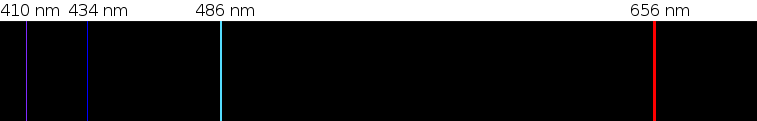
\includegraphics[width=0.9\textwidth]{Hspec}
	\caption{The visible emission spectrum of hydrogen\footnotemark.}
	\label{Hspec}
\end{center}
\end{figure}
\footnotetext{\url{www.commons.wikimedia.org/wiki/File:Emission_spectrum-H_labeled.svg}}
Another important line in radio astronomy is the 21cm hydrogen line. This line is a transition between two hyperfine states of neutral hydrogen and when a electron transits between these levels a photon of wavelength 21cm ($\sim$ 1.42 GHz) is emitted, hence the name. line emission can be used for determining velocities by using how much the line has been red shifted from its original wavelength, but the 21cm line is useful because it is not readily absorbed by clouds of gases.\\
\subsubsection*{Continuum Emission}
Continuum emission is radio emission that is emitted over a range of wavelengths rather than discretely like line emission. Continuum emission usually occurs with free particles, such as in plasma or gases.  There are several types of this emission however the important ones to mention for this project are Free Free emission and Synchrotron radiation.\\

Free-Free emission, is the process of a electron being deflected by an ion's electric field (accelerating it) which causes emission of photons. The electron remains free both before and after the interaction. The emission is usually produced from ionized hydrogen (HII) regions and the electron is free before and after the interaction hence the name.\\

Synchrotron radiation is important as it is a dominant source of radio emission (Ginzburg and Syrovtaskii 1965). Synchrotron occurs when relativistic electrons are accelerated by magnetic fields. This causes emissions of photons in the perpendicular direction to the acceleration which is then received by observers on Earth in the radio band. An example of this mechanic can be seen in Figure \ref{sync}.\\
\begin{figure}[H]
\begin{center}
	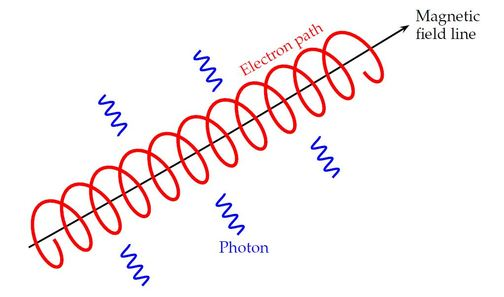
\includegraphics[width=0.7\textwidth]{sync}
	\caption{Diagram of how synchrotron radiation is emitted via electron spiraling around magnetic field\footnotemark. }
	\label{sync}
\end{center}
\end{figure}
\footnotetext{\url{www.cosmicriver.net/blog/synchrotron-radiation-diagram}}
These emissions allow us to see some interesting and unique objects in the radio regime and these sources can be expanded upon under two categories: Extra-Galactic and Galactic sources.


\subsubsection{Extra-Galactic Sources}
Extra-Galactic sources are sources which are not within our galaxy, the main type of radio source we see in this group are active galaxies. alpha galaxies are galaxies that are host to a active Galactic Nucleus (AGN). An AGN is a compact object at the center of a galaxy that has very large luminosity, up to 1000 times the luminosity of an average galaxy. The AGN's luminosity is powered by accretion of matter onto a Super Massive Black Hole (SMBH). The structure of a AGN can be seen in Figure \ref{agnstruc}, the SMBH is surrounded by an accretion disk which is fed by a torus of matter. The figure also shows two regions called the Broad line Region (BLR) and the Narrow line Region (NLR). The BLR is closer to the SMBH and the material is rotating around the black hole at high speeds ($\sim$10,000 km/s). This means that the spectral lines are broadened by a Doppler shift from the rotation. NLR are further away from the SMBH and do not rotate as quickly ($\sim$ 500 km/s), so the matter does not experience the same magnitude of Doppler shift and so the spectral lines are narrower than those emitted from the BLR.

\begin{figure}[H]
\begin{center}
	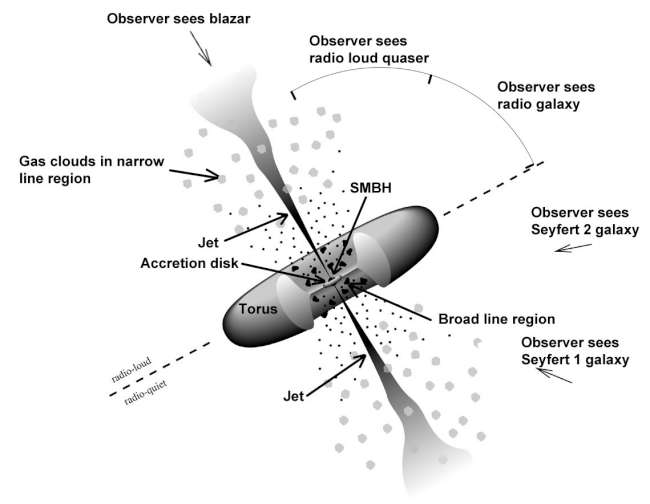
\includegraphics[width=0.75\textwidth]{SMBH}
	\caption{Structure of AGN. Figure shows the Narrow and Broad line regions, jet, torus and Super Massive Black Hole (SMBH) as well as the some of the radio loud/quiet classifications\footnotemark.}
	\label{agnstruc}
\end{center}
\end{figure}
\footnotetext{\url{www.kalataloetal.blogspot.com/2015/11/}}
Figure \ref{agnstruc} also shows the two sub-groups of AGN are radio-quiet AGN (bottom half) and radio-loud AGN (top half). Of all the AGN in our observable Universe, only $\sim$10\% are active within the radio portion of the EM spectrum. This subset of AGN has been further broken down within the literature into radio quiet and radio loud AGN which refers to their radio luminosities. We focus primarily on radio loud AGN as these produce the largest radio luminosities observed.

\begin{figure}[H]
\begin{center}
	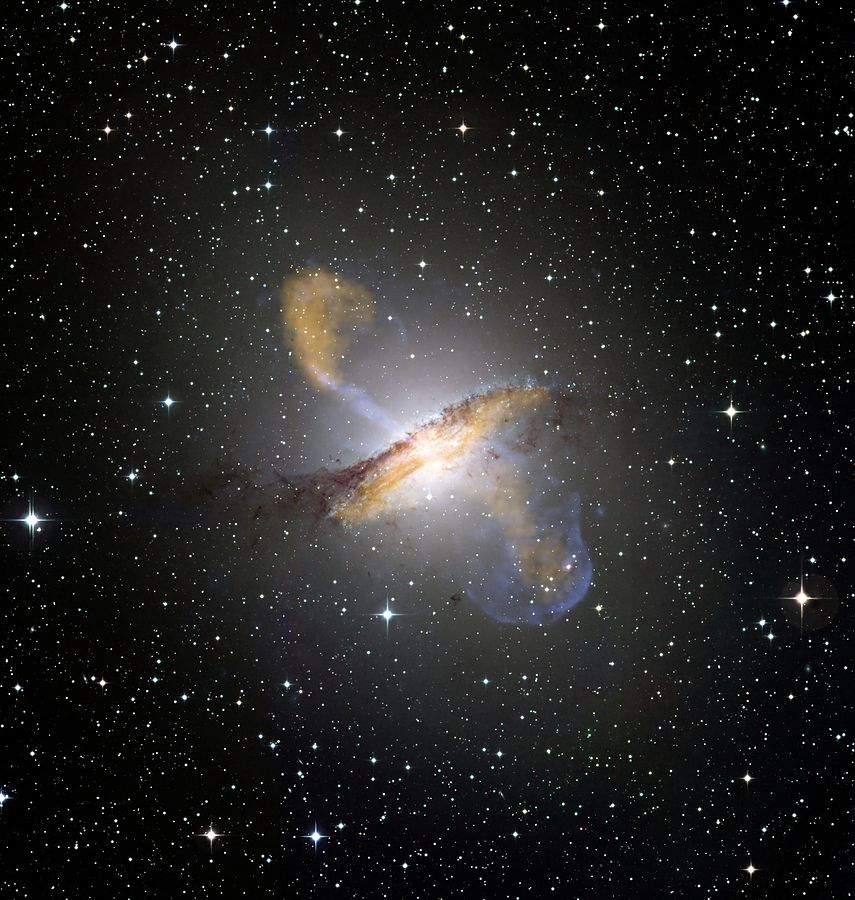
\includegraphics[width=0.5\textwidth]{CA}
	\caption{The active radio galaxy Centaurus A with radio jets seen being ejected by the AGN. Image composed of optical, xray (blue) and submillimetre (orange) spectrums\footnotemark.}
	\label{agn}
\end{center}
\end{figure}
\footnotetext{\url{www.eso.org/public/images/eso0903a/}}
Radio Galaxies (RGs), blazars and radio-loud quasars are all types of radio loud AGN. The main reason that these objects are loud is due to the jets that they produce being significantly luminous in the radio regime. These jets are highly collimated, high energy particles bound by magnetic field being channeled out of the AGN. The jets emits radio emission via the synchrotron process mentioned in Section \ref{radio} The difference between a blazar and RG is actually just a difference in viewing angle, a blazar's jet is pointed directly at our line of sight whereas a RG's is not.\\

It is important to note and compare AGN against Star Forming Galaxies (SFGs). SFGs are not as luminous as active galaxies, the main source of luminosity is generated by the stars themselves, rather than the accretion of matter onto a black hole at the center. A image of the SFG NGC 4414 is given in Figure \ref{sfg} for comparison to the AGN shown in Figure \ref{agn}.
\begin{figure}[H]
\begin{center}
	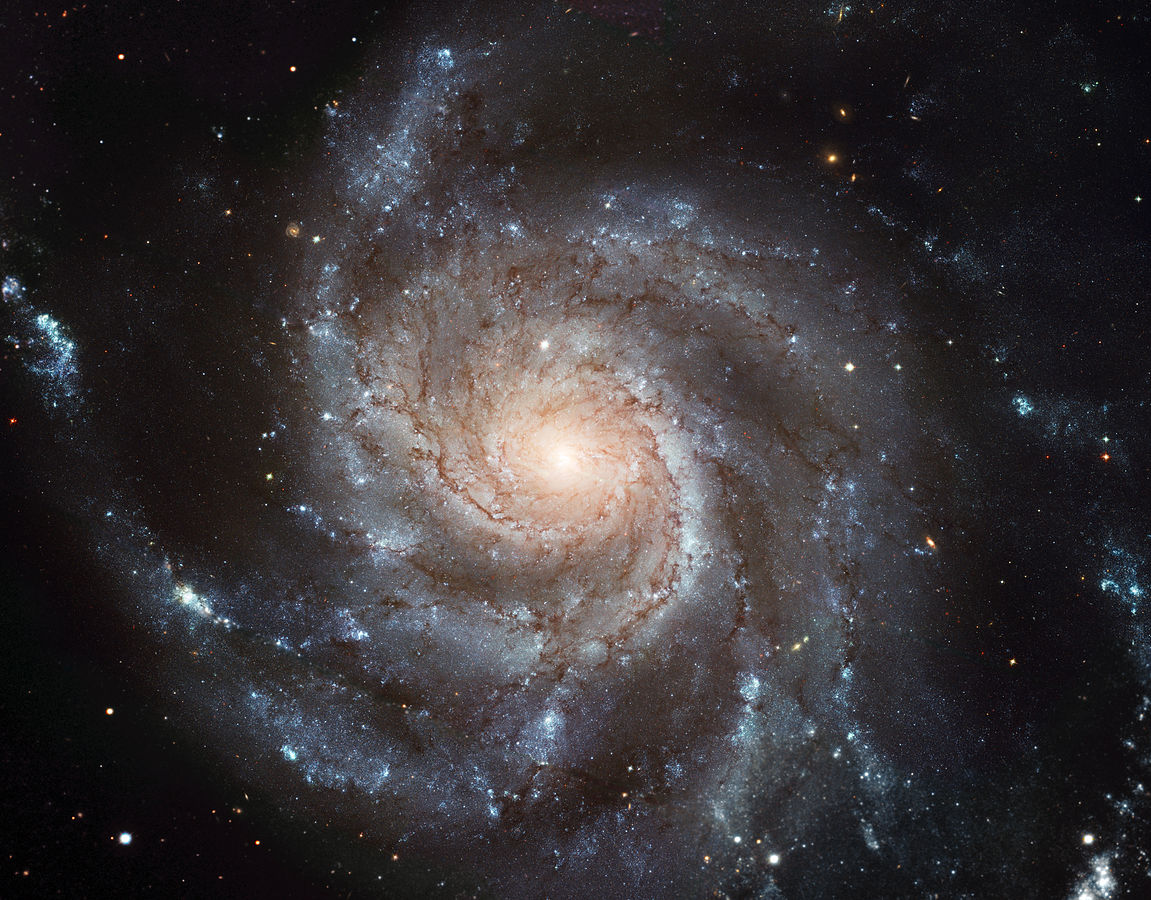
\includegraphics[width=0.55\textwidth]{M101}
	\caption{Example of Star Forming Galaxy - NGC 4414\footnotemark.}
	\label{sfg}
\end{center}
\end{figure}
\footnotetext{\url{www.hubblesite.org/image/1865/news_release/2006-10.}}
One of the interesting things about RGs is the morphology of jets, as seen in Figure \ref{fr} there are different components: the jet itself, lobes, hot spots and plumes. We can use these features to split RGs into two different categories FRI and FRII. FRI galaxies have bright inner jets (Figure \ref{fr} left) whereas FRII are fainter in the centre but have brighter hot spot where the jet `terminates' (Figure \ref{fr} right). The `hot spot' is not hot in terms of temperature but rather hot in terms of more radio waves being emitted from that region. The strength of the jet as well as the surrounding medium have impacts on the morphology and classifications of the RGs. FRII galaxies have intrinsically more powerful jets than FRI, which is in part responsible for the clear distinction between the FRI and FRII morphology; in particular whether the jet travels relatively undisturbed or whether the jet mixes with the environment shortly after leaving the host galaxy. This is further influenced by the environmental properties within which these radio galaxies are populated. Denser mediums can suppress, bend and deform the radio lobes which has been linked to the FRI/FRII distinction as well as other peculiar RG types such as Wide Angled Tail (WAT) and Head Tail (HT) sources.
\begin{figure}[H]
\centering
\begin{subfigure}[b]{0.49\textwidth}
	\centering
	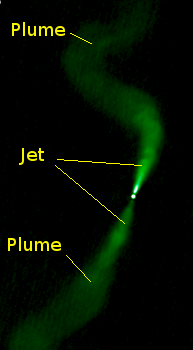
\includegraphics[height=\textwidth]{fr2}
\end{subfigure}
\begin{subfigure}[b]{0.49\textwidth}
	\centering
	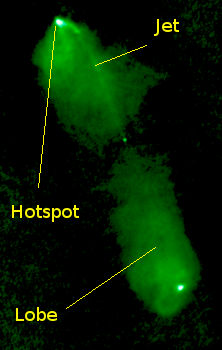
\includegraphics[height=\textwidth]{fr1}
\end{subfigure}

\caption{Labelled diagram of radio galaxies. Left: FRI type galaxy 3C31, Right: FRII type galaxy 3C98\footnotemark.}
\label{fr}
\end{figure}
\footnotetext{\url{www.en.wikipedia.org/wiki/Radio_galaxy}}

\subsubsection{Galactic Sources}
The other subgroup of radio sources are ones that are within our Galaxy. The milky way contains lots of interesting sources in the radio regime such as Sagittarius A* the supermassive black hole at the center, pulsars, super nova remnants (SNRs) and x-ray binaries.\\

When a supernova occurs the matter is ejected outwards from the core of the host star. This matter is ejected in a shock front sweeping up matter as it passes. The left over structure is what we refer to as a SNR and it is bounded by this continually expanding shock front. These SNRs are detected in the radio regime via synchrotron radiation (\citet{Mayer}).\\

The pulsar is another object that we see emitting in the radio spectrum. A pulsar is a rapidly rotating neutron star that produces beams of synchrotron radiation along its magnetic poles as it rotates.  The beams of radiation sweep around the pulsar like a lighthouse and we see pulses of radiation as they cross our line of sight. These pulses of radiation are very regular and only last a short amount of time, from milliseconds to a couple of seconds. A pulsar is created when a star's core of certain mass ($\sim2.5-3 M_\odot$) collapses to form a much smaller radius neutron star supported by neutron degeneracy pressure (Camenzind 2007 \citet{Camezind}). This drastic change in radius and the fact that angular momentum is conserved means that the neutron star rotates much faster than its progenitor making it incredibly stable. This stability and repeatability of pulsars is what makes them very interesting objects, because of this pulsars are often used to test other things. An example of this is using pulsars to measure electron density between the pulsar and the observer. Another more exciting example is the idea that a pulsar timing array could be created to detect very low frequency gravitational waves - a galactic interferometer.\\

The final object that will be mentioned is X-ray binaries. These are binaries between either a black hole or neutron star and a donor star which accretes matter onto the black hole or neutron star. These emit mainly in the X-ray but also have a strong component in the radio due to synchrotron radiation.
\begin{figure}[H]
\begin{center}
	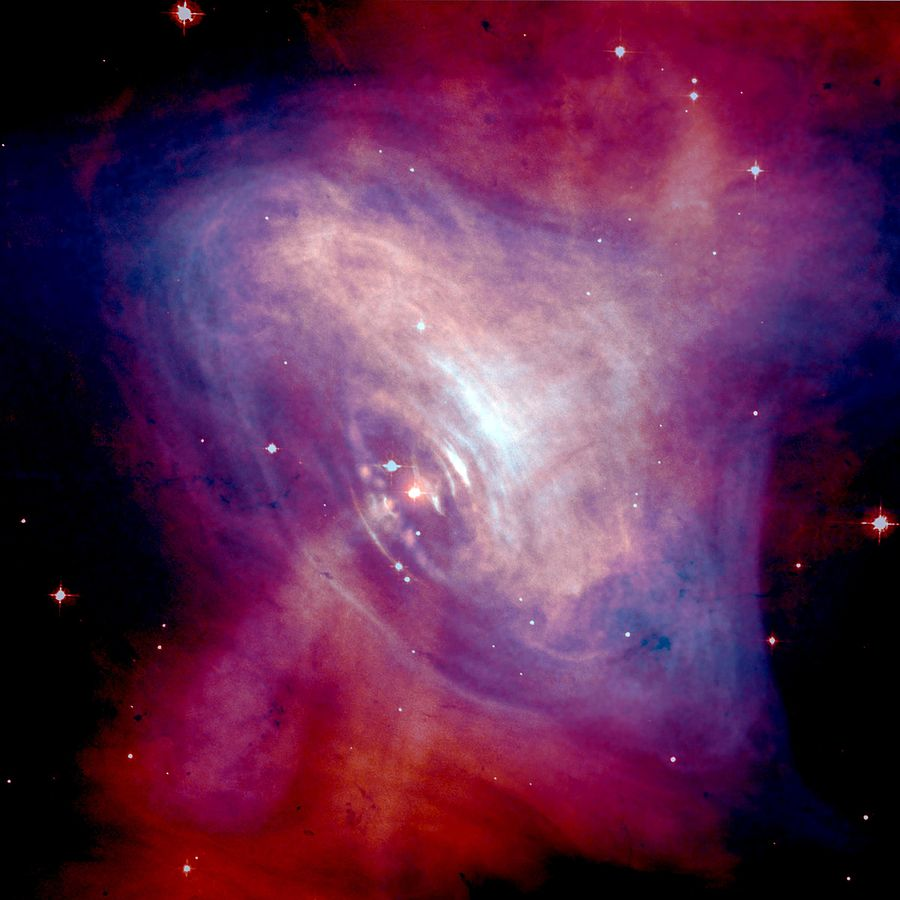
\includegraphics[width=0.5\textwidth]{pulsar}
	\caption{Crab pulsar inside the Crab Nebular. Optical in Red, X-ray in blue\footnotemark.}
	\label{pulsar}
\end{center}
\end{figure}
\footnotetext{\url{www.hubblesite.org/image/1248/news_release/2002-24}}
One thing to note about these radio sources is that when observing them some objects will be compact (point like) or have compact emission sites meaning that we can not resolve them with telescopes easily because they appear so small. Objects such as AGN, and pulsars are considered compact. 
However some objects will be extended and are more easily resolved, because their emission is spread over a larger area. Objects such as SNRs and radio galaxies with jets are considered extended. However it is not always so black and white, there are overlaps as some extended objects can regions of compactness. This is important to consider when observing objects mainly regarding scintillation as a objects angular size or compactness can affect whether it scintillates or not.

\subsection{Variability}
Variability is the change in flux over time of a object, this variation in flux can occur at different time scales ranging from days to decades. The two main groups of variability are intrinsic and extrinsic. Intrinsic variability is when the actual object is varying over a given time and causes the flux produced to change.\\

Variability can give information information depending on the type of variability that is observed. If a  exhibits intrinsic variability we can infer properties of the object or even events that are occurring at the object. Intrinsic variability has lots of different objects that vary on a wide range of timescales as seen in Figure \ref{intrinsic}.
\begin{figure}[H]
\begin{center}
	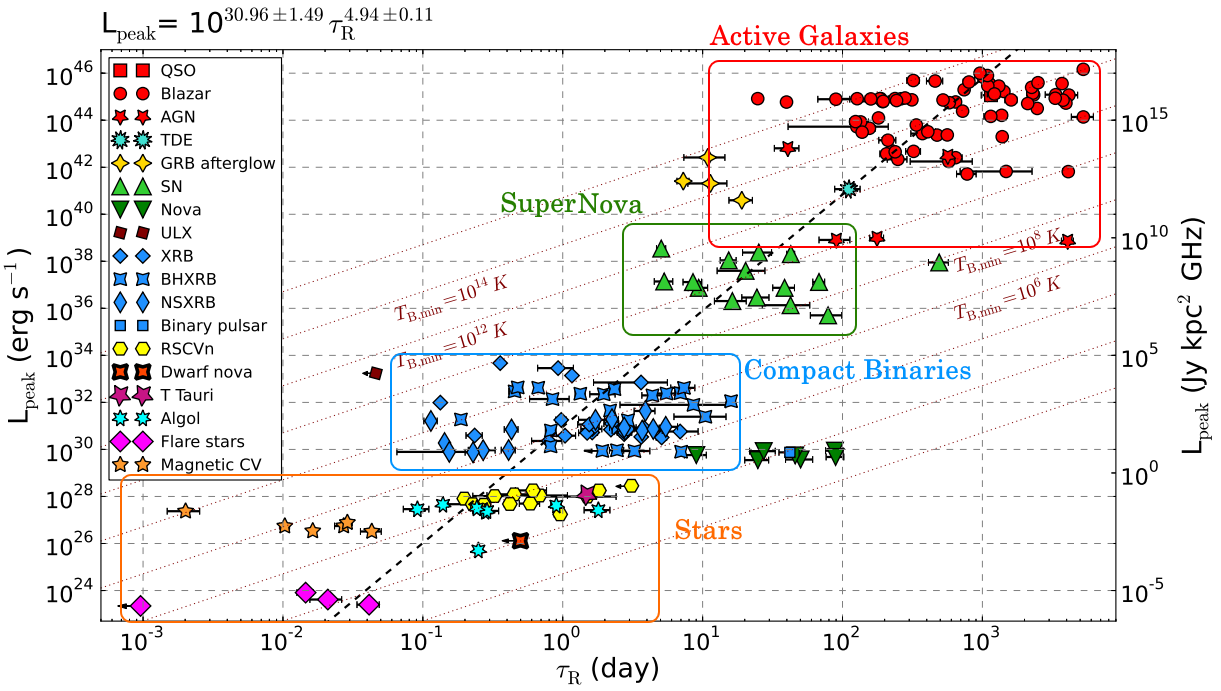
\includegraphics[width=\textwidth]{intrin3}
	\caption{Plot showing Luminosity of different objects versus the intrinsic variability timescale. Also shown are 4 distinct groups of objects. In red there are the radio and active galaxies, green are supernovaes, blue are the binaries and x-ray binaries, in orange are the variable stars. Original from \citet{Pietka}}
	\label{intrinsic}
\end{center}
\end{figure}
Figure \ref{intrinsic} shows the 4 distinct groups of objects, however it is also important to look at the timescale that these objects are varying on. In red there are the active galaxies with timescales of $\sim 1000$ days. Green are supernovaes with timescales of  $\sim 50$ days. Blue are the binaries and x-ray binaries with timescale  $\sim 1$ day. Finally in orange are the variable stars which have timescales of 1 day or less. Not shown in the figure are pulsars that are very far to the left of the diagram with variable timescales that are orders of magnitude smaller. In this project the main objects that we will be measuring the variability of, is the active galaxies and they are only intrinsically varying on timescales of 100-1000 days this means that we will not see them varying in images taken over minutes-days. Therefore the main contribution of these objects variability must be the extrinsic variability.\\

Extrinsic variability is when the signal from a object is changed on its way to the observer, this changes the amount of flux the observer receives. The major cause of extrinsic variability is the intervening material between object and observer interacting or interfering with the signal, this is called scintillation and will be discussed further in Section \ref{scint} but first we will talk about our Galaxy's structure.\\

\subsection{Milky Way Structure}
When we observe anything in space, whether it be the Sun, a neighbouring star or Galaxy we have to take into consideration the intervening material and what effects the journey has on the received signal. There are several different intervening materials that we can consider: Ionosphere, the upper atmosphere around Earth. Interplanetary medium (IPM), mainly from flares around a host star. Interstellar medium (ISM), the medium in between stars that is around the whole Galaxy. Intergalactic medium (IGM), the material between galaxies. However not all media are as important as each other due to different timescales that each medium works on. The medium that has the greatest effect is the ISM and so we will focus on its structure and density through our Galaxy.\\

When looking into the Milky Way it is important to think about its structure. The Earth exists in a spiral Galaxy, which we can simply model as a flattened ellipsoid, similarly shaped to a pancake (Figure \ref{MWS}). When we are looking into the galactic plane of the Galaxy we are looking at a 2D ellipse shaped slice of the Galaxy. When looking at the densities in this slice we can only measure along the line of sight that we are observing at. There are many different measures we can use when looking into the Galaxy, each of which can be used to observe or look at different things or even see past material that might be in the way. An interesting measure to take is the Hydrogen alpha density.\\
\begin{figure}[H]
\begin{center}
	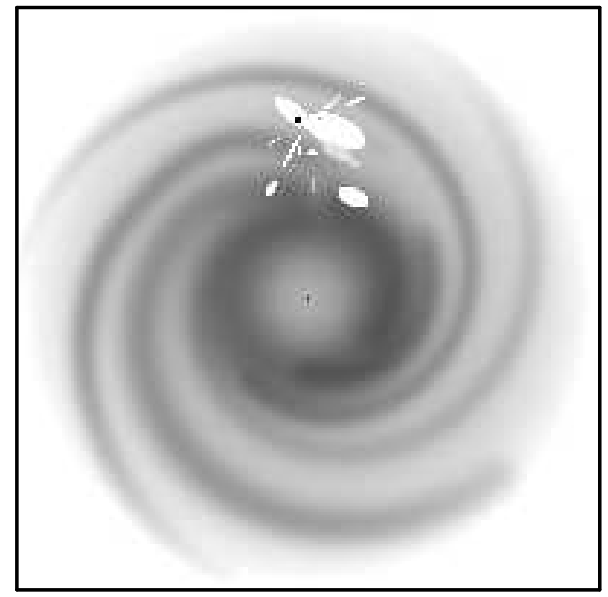
\includegraphics[width=0.6\textwidth]{MWS}
	\caption{Shows the model used for structure of milky way, white patches shows line of sights where structure is better known. (Cordes \& Lazio 2003.)}
	\label{MWS}
\end{center}
\end{figure}
%\begin{figure}[H]
%	\begin{center}
%		\includegraphics[width=\textwidth]{comp}
%		\caption{Plot showing comparison images of the galactic plane in four different wavelengths of observation: Optical, Near-Infrared, Infrared and Submillimetre.}
%		\label{comp}
%	\end{center}
%\end{figure}
\subsubsection{Using Hydrogen alpha to Map Density}
The H$\alpha$ line is a tracer for regions of ionizing hydrogen which usually contain a lot of matter. H$\alpha$ measures the emission down the line of sight, this is called the emission measure (EM). H$\alpha$ can be used to map the density of electrons along the line of sight. Using theory about how these electrons are distributed and their associated turbulence discussed in the Cordes 2003 paper. We can then convert the EM given by the H$\alpha$ intensity to  the scattering measure:
\[ \ce{SM}= \frac{\ce{I_{H\alpha}}}{198} \ce{T_4^{0.9}} \frac{\epsilon^2}{1+\epsilon^2}l_0^{-2/3} \]
This scattering measure can then be used to calculate other parameters used to analyse the variability, this is expanded upon in the calculation section. Their are limits to this though, the H$\alpha$ does not measure all of the matter down the line of sight but makes a good estimation towards it. From this it then follows that if you can create a map of the H$\alpha$ in the Galaxy then you could predict what the variability should be based upon the coordinates of the objects on the galactic plane. A map of the Hydrogen alpha can be seen in Figure \ref{Halpha}. 


H$\alpha$ measures the emission down the line of sight, this is called the emission measure (EM). H$\alpha$ can be used to map the density of electrons along the line of sight. Using theory about how these electrons are distributed and their associated turbulence, discussed in the Cordes 2003 paper, We can then convert the EM given by the H$\alpha$ intensity to the scattering measure:

%H\alpha measures the number of photons emitted along the line of sight, this is the emission measure. Since H\alpha is a free-bound transition this maps on to the density of electrons are along the line of sight. If we then add some theory about how these electrons are distributed and the nature of their turbulence, then you can convert the H\alpha (or EM) in to the scattering measure..

\begin{figure}[H]
\begin{center}
	%\includegraphics[width=0.78\textwidth]{GLEAM_Data}
	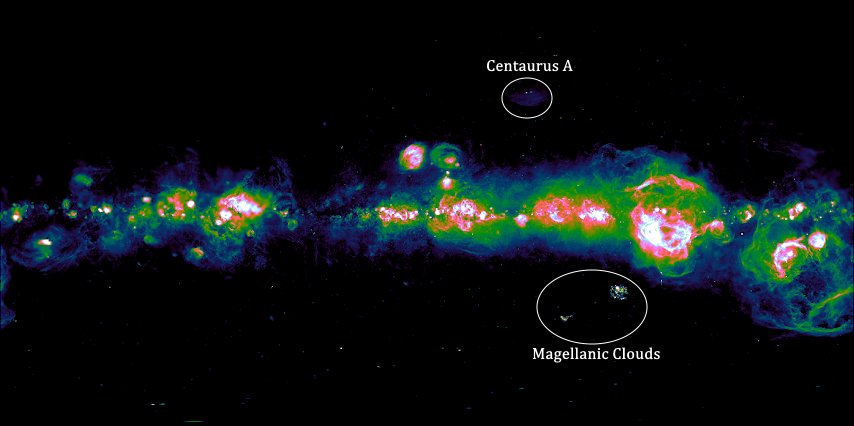
\includegraphics[width=0.78\textwidth]{Ha1_annotated}
	%\includegraphics[width=0.78\textwidth]{gp_r2GHz}
	%\includegraphics[width=0.78\textwidth]{Ha4}
	\caption{Hydrogen alpha map of the Milky Way's galactic plane. Intensity of H$\alpha$ ranges from lowest - black to highest - white. Also seen are the extra galactic objects the large and small Magellanic clouds as well as the radio galaxy Centaurus A.}
	\label{Halpha}
\end{center}
\end{figure}
So the question now is how does matter down the line of sight contribute to how a object varies, and how does the amount of matter affect this variation. As mentioned earlier these effects that vary the flux are called Scintillation.

\subsection{Scintillation}\label{scint}
When viewing a signal from a object, the signal has to travel some distance through space to arrive at us. While traveling the signal can experience several different effects which can be seen by an observer. These can be summarised into two main categories: Wave distortion and path length changes, the effects of both are further described below.

\subsubsection{Wave Distortion by the ISM}\label{ISM}
The ISM is a ionized plasma which interacts with signals that pass through it. These effects are particularly important when viewing object at different frequencies as the interactions of the ISM with propagating waves are heavily frequency dependent. The ISM is turbulent and contains many inhomogeneities and when radiation propagates through these inhomogeneities we get scintillation and scattering effects.
To simplify the model of the ISM, in 1968 Scheuer modeled the ISM as a ``thin screen model". This was done by collapsing all the inhomogeneities onto a thin screen some distance (D) between the target and observer (Scheuer 1968). This model can be used to predict what effects should happen to the traveling radiation. Scintillation and scattering are derived from the same effect: wave-fronts being distorted by the ISM (Figure \ref{path}).
\begin{figure}[H]
    \centering 
    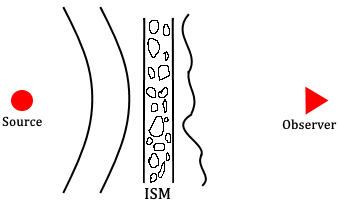
\includegraphics[width=0.7\textwidth]{thinscreen}
    \caption{Thin screen model. The diagram shows the effect a inhomogeneous medium, like the ISM, affects a wave when it passes through it. A simple model can be used to help predict these effects, called the thin screen model.}
    \label{path}
\end{figure}

When the radiation passes through the thin screen the wavefronts are distorted changing the phase angle slightly. These small changes cause the waves to interfere with one another either constructively or destructively. This interference causes fluctuations in intensity which can be seen by an observer (Lorimer and Kramer 2005). The variation due to this can be quantified as the diffractive length scale ($r_{\ce{diff}}$). This length scale is defined as the transverse seperation across a wavefront that the root mean square (RMS) of the phase difference is equal to one radian. One radian is the limit where these phase fluctuations of the wavefront are coherent with one another.

\subsubsection{Path Length Variation}\label{plen}
The other type of wave change is caused by a change in path length. This is when you have a object emitting a signal some distance away from a receiver sometimes the signal does not travel directly from the receiver to the observer, often the signal will be reflected towards the receiver (Figure \ref{slic}). A Fresnel zone is defined based upon what phase shift the reflected signal has upon arriving at the receiver due to a change in path length of the signal. The first Fresnel zone is the zone we are most interested in as it is where the phase shift contributes mostly coherently to the signal, the zone are in forms of prolate ellipsoid's around the receiver and the object seen in Figure \ref{elips}. Zones outside of the first are not as important as the effects drop off dramatically the further away from the main signal the zone gets.
\begin{figure}[H]
\centering 
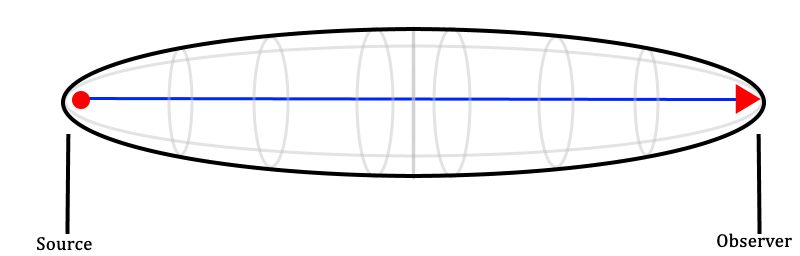
\includegraphics[width=0.7\textwidth]{Fres_elips}
\caption{The ellipsoid of the first Fresnel zone.}
\label{elips}
\end{figure}
We can see that if we take a 2D slice of this ellipsoid we can have a large number of reflections happening at different points along the ellipse demonstrated in Figure \ref{slic} we can also imagine that we can rotate this slice and get the same range of signals reflecting towards the observer.
\begin{figure}[H]
\centering 
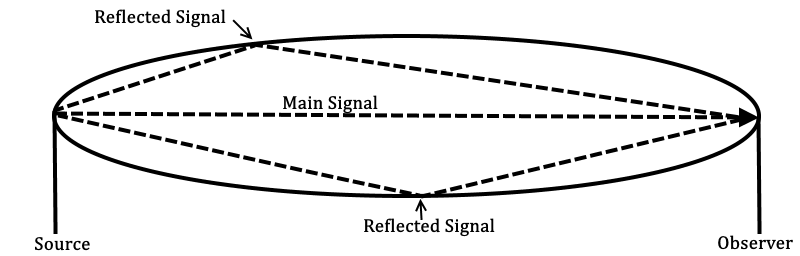
\includegraphics[width=0.7\textwidth]{Fres_slice}
\caption{A 2D slice of the Fresnel Zone ellipsoid showing how the main signal travels directly to the observer whereas the reflected signals have a path length increase. Also shows that we can have many different signals reflecting at different points along the Fresnel Zone.}
\label{slic}
\end{figure}
As the observer when we look at the object we can see all of these signals coming from the first Fresnel zone as a circle, like the grey ones we see in Figure \ref{elips}. From this the first Fresnel zone can be defined as having a Fresnel scale ($r_F$) at a distance (D) away from the object (Figure \ref{circle}). 
\begin{equation}
r_F=\sqrt[]{\dfrac{\lambda D}{2\pi}}
\label{eq:rf}
\end{equation}
Where $\lambda$ is the wavelength of the radiation and D is the distance to the screen. From this and the distance the Fresnel angle can also be calculated.
\begin{figure}[H]
\centering 
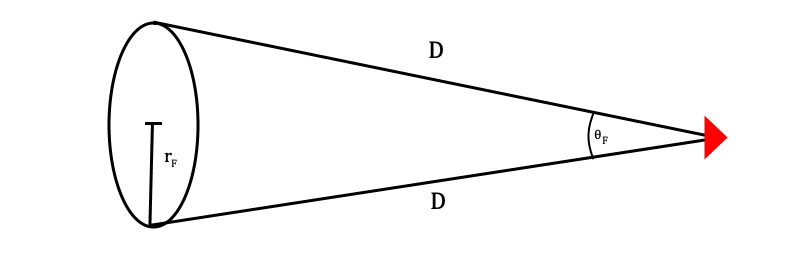
\includegraphics[width=0.7\textwidth]{Fres_circle}
\caption{Another 2D cut but in a different plane of the ellipsoid. The circle is what we see when looking at the object as it is where all the signals must pass through in the first Fresnel zone. The diagram also shows the defined quantities of the Fresnel scale, and the Angular size of the Fresnel zone.}
\label{circle}
\end{figure}
We can also calculate the angular size of this zone using basic trigonometry and assuming that the angle is very small gives the equation for the Fresnel angle ($\theta_F$):
\begin{equation}
    \theta_F=\dfrac{r_F}{D}
    \label{eq:thetaf}
\end{equation}
Using the definitions from above for path length variations and wave distortion we can define the boundaries between weak and strong scattering stated by \citet{Narayan} as:\\

Weak: $r_{\ce{diff}} \gg r_{F}$ the random phase fluctuations in the first Fresnel zone are small and so the weak fluctuations due to the distorted wavefront are seen by the observer.\\

Strong: $r_{\ce{diff}} \ll r_{F}$ the random phase fluctuations due to the scattering screen vary by many radians over the first Fresnel zone making it irrelevant. This means that $r_{\ce{diff}}$ becomes the length scale of the coherent patch.\\


\subsubsection{Weak \& Strong Scintillation}
As defined before we have two different regions of scattering, weak and strong. In weak scattering small variation of the flux occur mainly due to the phase fluctuations focusing/defocusing with length scales of approximately the Fresnel scale. A modulation index ($m_p$) can be defined as the root mean square amplitude of the flux scintillation divided by its mean. For a point object whose Fresnel angle ($\theta_F$) is less than that of the object's angular size ($\theta_S$) the modulation index for weak scattering is:
\begin{equation}
    m_{p}=(r_{F}/r_{\ce{diff}})^{\frac{5}{6}}
\end{equation}
In strong scattering there are two different regimes called diffractive and refractive scintillation. 
\begin{figure}[H]
\begin{center}
	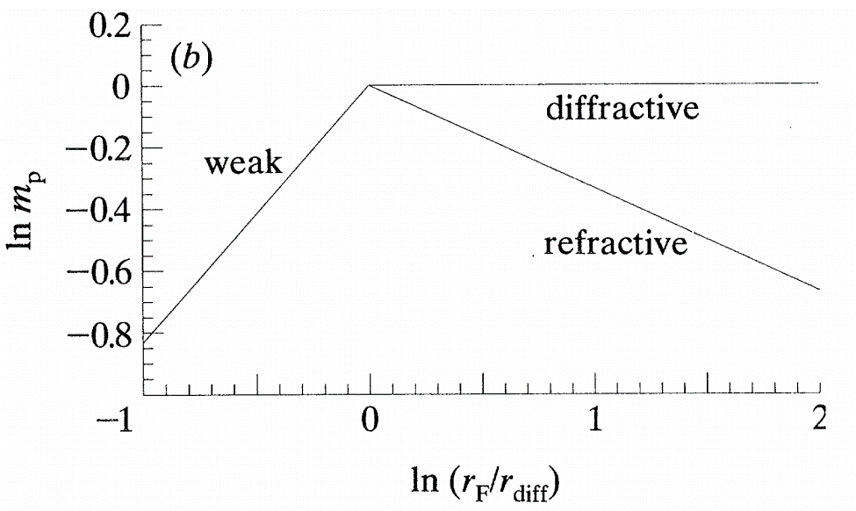
\includegraphics[width=0.7\textwidth]{scatt1}
	\caption{The plot of the modulation index which shows how the regimes are split up by there fresnel scale and diffractive length scale ratio (Narayan 1992).}
	\label{scatt}
\end{center}
\end{figure}
\subsubsection{Refractive vs Diffractive} \label{RvD}
Diffractive scintillation occurs on length-scales of $r_{\ce{diff}}$ and refractive occurs on times scales of $r_{\ce{ref}}$. We can use the former to calculate the latter via the following equation:
\[ r_{\ce{ref}} = r_{F}^{2}/r_{\ce{diff}}\gg r_{\ce{diff}} \]
Refractive scintillation has smaller flux fluctuations than diffrative scintillation but occurs on a much longer length-scale. Weak and strong scattering are both important and one should not overlook them without consideration, however for this project we are only going to care about strong refractive Scintillation. We are in the strong regime due to the frequency that we are observing between ($\sim$100MHz - 1GHz) and also the medium we are looking through (ISM) which limits us to the strong regime also seen in Figure \ref{scatt} (Narayn 1992). The NE2001 (Cordes \& Lazio 2003) paper already models the diffractive regime, whereas there is no major model for the refractive yet. This is why we focus on the refractive as it is much more useful for lower time and frequency resolution and we can create a model for this regime. This is because we are creating images which are being averaged over approximately two minutes worth of time and about 1.28 MHz, the diffractive time scale is much smaller than this which means that it is getting averaged over, making it useless. The diffractive regime is better used for high time and high frequency resolution which is why it is very useful for pulsar observations.\\

From this point we have two options with what to do with this information about scintillation. The first option is that we could measure variable object and work backwards to investigate the intervening material between us, the observer, and the object. The second is to use models/assumptions of the turbulence and distribution of material in the line of sight of the object to predict variability. The first option requires a lot of time and line of sight measurements, while the second can be done using easily obtainable models that have extensive background behind them. In this dissertation we have chosen to pursue the second option. 
\subsection{Previous Works}
As mentioned in Section \ref{RvD} the NE2001 model is used mainly in pulsar work as it can produce the distribution for free electrons, model fluctuation in electron density, as well as other parameters explained in NE2001 I paper. The NE2001 model builds upon Taylor \& Cordes 1993 \citet{Taylor} model by implementing newer models with larger amounts of data and new dispersion and scattering measurements. They take data from all available pulsar dispersion measures available at the time as well as including new and more accurate distance measurements from HI observations and parallax measurements. Cordes \& Lazio 2003 \citet{Cordes} contains the full details of the model.\\

Dr Paul Hancock already knew of this model and thought it would be useful to create a model that does something similar but for refractive scintillation so he started the SM2017 model on which this work is built upon. This model uses the density and distribution models from NE2001 as a base. The SM2017 model then takes the basic enough starting point of the H$\alpha$ distribution in the galactic plane and calculates various quantities which can be used to analyse the variability of a object or objects at given coordinates. However this is still quite simple and some more physics and parameters could easily be added to improve the model to give a reasonable measure of uncertainty. The current state of the SM2017 model is show in Figure \ref{SM2017}.
\begin{figure}[H]
\begin{center}
	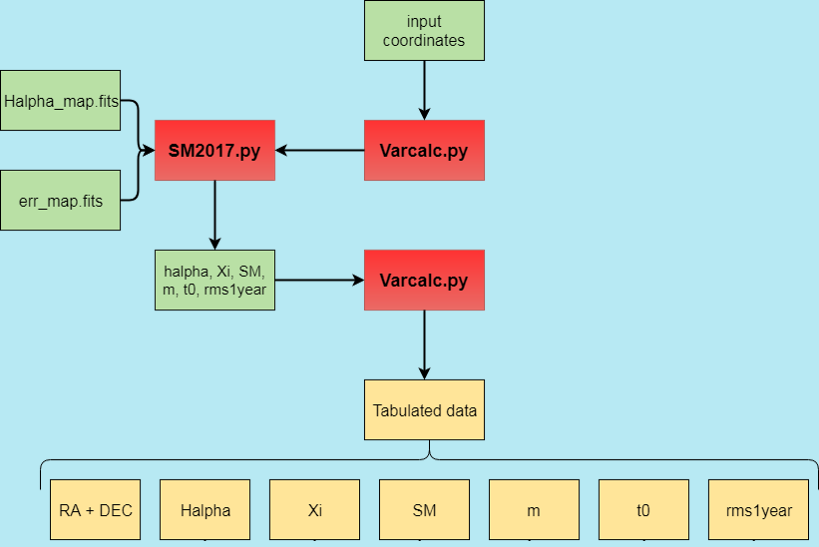
\includegraphics[width=0.8\textwidth]{SM2017_old}
	\caption{The SM2017 model create by Dr. Paul Hancock, showing the flowchart of how the program takes initial input coordinates and generates variability statistics.}
	\label{SM2017}
\end{center}
\end{figure}
\subsection{Aims and Scope}
The motivation behind this project was to create a model that can take the positions of a group of sources and to use some fairly simple assumptions and measurements to predict variability for these sources. I started with a base model created by my supervisor and over the course of the project the model will have more components added to it, to make it more reliable and accurate until it is usable and available to a wider audience. Previous models predicted single source statistics we want to be able to produce population statistics, which is what a real survey would see. This means that we have to include various parameters to make the model viable such as correct clustering and distributions.\\

The scope for this work is to be able to simulate object points in a given area of sky provided by the user. The program will then take given parameters and generate a simulation of the objects and then calculate variability parameters. This would be done enough times that the distribution of how the objects were varying over time could be calculated to give the actual variability back to the user. The main improvements upon the SM2017 model will be made in parameters applied to generating the objects. Source counts, objects clustering, two point correlation function would all be good to include as they allow for a more realistic distribution of generated objects. Another aspect to look at including in the model would be to generate compact and extended objects and use the different calculations required to determine variability. All of these would ideally be implemented into the SM2017 model to get a realistic simulation of the variability. A flow chart of this can be seen in Figure \ref{VarSim}.\\

In future the model will be able to take a survey and return the variability expected from scintillation alone, allowing the researcher to tell if there are any interesting variable sources within this survey, or have a baseline measurement for what variability in the flux observed would be.
\begin{figure}[H]
\begin{center}
	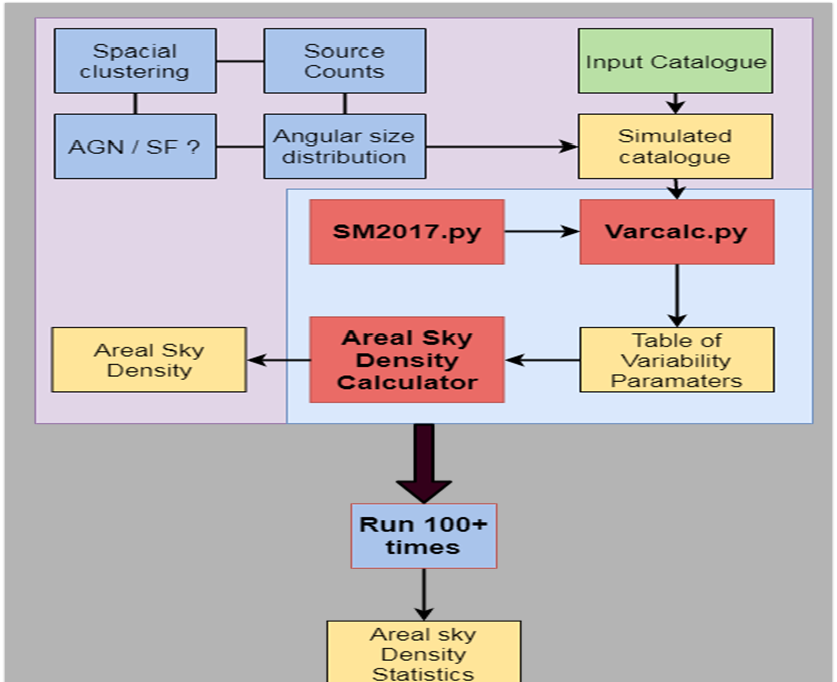
\includegraphics[width=0.7\textwidth]{VarSim}
	\caption{A flow chart representing how the final model should work with the SM2017 model from Figure \ref{SM2017} shown in the blue box.}
	\label{VarSim}
\end{center}
\end{figure}



			
			
			
			
\end{document}

